\documentclass[8pt,a4paper,compress]{beamer}

\usepackage{/home/siyer/lib/slides}

\title{Defining Functions}
\date{}

\begin{document}
\begin{frame}
\vfill
\titlepage
\end{frame}

\begin{frame}
\frametitle{Outline}
\tableofcontents
\end{frame}

\section{Using and Defining Functions}
\begin{frame}[fragile]
\pause

Functions allow us to
\begin{itemize}
\item Transfer control back and forth between different pieces of code
\item Clearly separate tasks within a program
\item Reuse code
\end{itemize}

\pause
\bigskip

Function definition in Python
\begin{lstlisting}[language={}]
def <name>(<parameter name>, <parameter name>, ...):
    <statement>
    <statement>
    ...
\end{lstlisting}

\pause
\bigskip

Anatomy of a function
\begin{itemize}
\item The first line, known as the signature, consists of the \lstinline{def} keyword, the function name, a sequence of zero or more parameter variables separated by commas and enclosed in parentheses, and a colon

\item The indented statements following the signature constitute the function body

\item The function body can contain a return statement, which transfers control to the point where the function was called and returns the result of the computation (aka the return value)
\end{itemize}
\end{frame}

\begin{frame}[fragile]
\pause

For example, the following function tests if the argument $N$ is prime

\begin{lstlisting}[language=Python]
def is_prime(N):
    if N < 2: 
        return False
    i = 2
    while i <= N / i:
        if N % i == 0:
            return False
        i += 1
    return True
\end{lstlisting}

\pause
\bigskip

A function call, such as \lstinline{is_prime(31)}, is its name followed by expressions that specify argument values in parentheses, separated by commas

\pause
\bigskip

When the function call is part of an expression, as in \lstinline{x = math.sqrt(3)}, the function computes a value that is used in place of the call in the expression

\pause
\bigskip

Otherwise, the function call is a statement that generally causes side effects, as in \lstinline{stdio.writeln('Hello, World')}
\end{frame}

\begin{frame}[fragile]
\pause

\begin{framed}
\tiny harmonicf.py:  Write to standard output the harmonic numbers specified as command-line arguments.
\end{framed}

\begin{lstlisting}[language=Python]
import stdio
import sys

def harmonic(n):
    total = 0.0
    for i in range(1, n + 1):
        total += 1.0 / float(i)
    return total

def main():
    stdio.writeln('in main()')
    for j in range(1, len(sys.argv)):
        arg = int(sys.argv[j])
        value = harmonic(arg)
        stdio.writeln(value)

if __name__ == '__main__':
    main()
\end{lstlisting}

\pause

\begin{lstlisting}[language={}]
$ python harmonicf.py 2
in main()
1.5
\end{lstlisting}

\pause
\bigskip

When a program is executed directly by the \lstinline{python} command (and not imported as a module via the \lstinline{import} statement), the program's \lstinline{__name__} attribute is set to \lstinline{'__main__'}

\begin{lstlisting}[language={}]
>>> import harmonicf
>>> 
>>> harmonicf.harmonic(4)
2.08333333333
\end{lstlisting}
\end{frame}

\begin{frame}[fragile]
\pause

A Python function can have more than one parameter variable, so it can be called with more than one argument
\begin{lstlisting}[language=Python]
def hypot(a, b):
    return math.sqrt(a * a + b * b)
\end{lstlisting}

\pause
\bigskip

We can define as many functions as we want in a \lstinline{.py} file
\begin{lstlisting}[language=Python]
def square(x):
    return x * x

def hypot(a, b):
    return math.sqrt(square(a) + square(b))
\end{lstlisting}

\pause
\bigskip

We can put \lstinline{return} statements in a function wherever we need them, as in the \lstinline{is_prime()} function

\pause
\bigskip

A function provides only one return value to the caller; more precisely, it returns a reference to one object

\pause
\bigskip

The scope of a function's local and parameter variables is limited to that function

\pause
\bigskip

The scope of a variable defined in global code --- known as a global variable --- is limited to the \lstinline{.py} file containing that variable
\end{frame}

\begin{frame}[fragile]
\pause

A function may designate an argument to be optional by specifying a default value for that argument

\pause
\bigskip

For example, the following function computes the $n$th generalized harmonic number of order $r$, $H_{n,r}=1+1/2^r+1/3^r+\cdots+1/n^r$

\begin{lstlisting}[language=Python]
def harmonic(n, r = 1):
    total = 0.0
    for i in range(1, n + 1):
        total += 1.0 / (i ** r)
    return total
\end{lstlisting}
With the above definition, \lstinline{harmonic(2, 2)} returns \lstinline{1.25}, while both \lstinline{harmonic(2, 1)} and \lstinline{harmonic(2)} return \lstinline{1.5}

\pause
\bigskip

Named arguments allow us to specify arguments to a function in any order

\pause
\bigskip

For example, the call \lstinline{harmonic(r = 2, n = 3)} is the same as the call \lstinline{harmonic(3, 2)}

\pause
\bigskip

Python supports functional polymorphism, which allows us to define a single function for use with objects of different types

\pause
\bigskip

For example, \lstinline{square()} when called with an integer argument, returns an integer, but when called with a float argument, returns a float
\end{frame}

\section{Implementing Mathematical Functions}

\begin{frame}[fragile]
\pause

\begin{minipage}{170pt}
The standard Gaussian probability density function (pdf) is characterized by the familiar bell-shaped curve defined by the formula $\phi(x)=e^{-x^2/2}/\sqrt{2\pi}$

\pause
\bigskip

The Gaussian pdf $\phi(x, \mu, \sigma)$ is the same as $\phi((x-\mu)/\sigma)/\sigma$

\pause
\bigskip

The standard Gaussian cumulative distribution function (cdf) $\Phi(z)$ is defined to be the area under the curve defined by $\phi(x)$ above the $x$-axis and to the left of the vertical line $x=z$ 

\pause
\bigskip

No formula is known for $\Phi(z)$, but it can be approximated as follows $$\Phi(z)=\frac{1}{2}+\phi(z)\big(z+\frac{z^3}{3}+\frac{z^5}{3\cdot 5}+\frac{z^7}{3\cdot 5\cdot 7}+\cdots\big )$$
\end{minipage}\hfill%
\begin{minipage}{130pt}
\begin{center}
\visible<2->{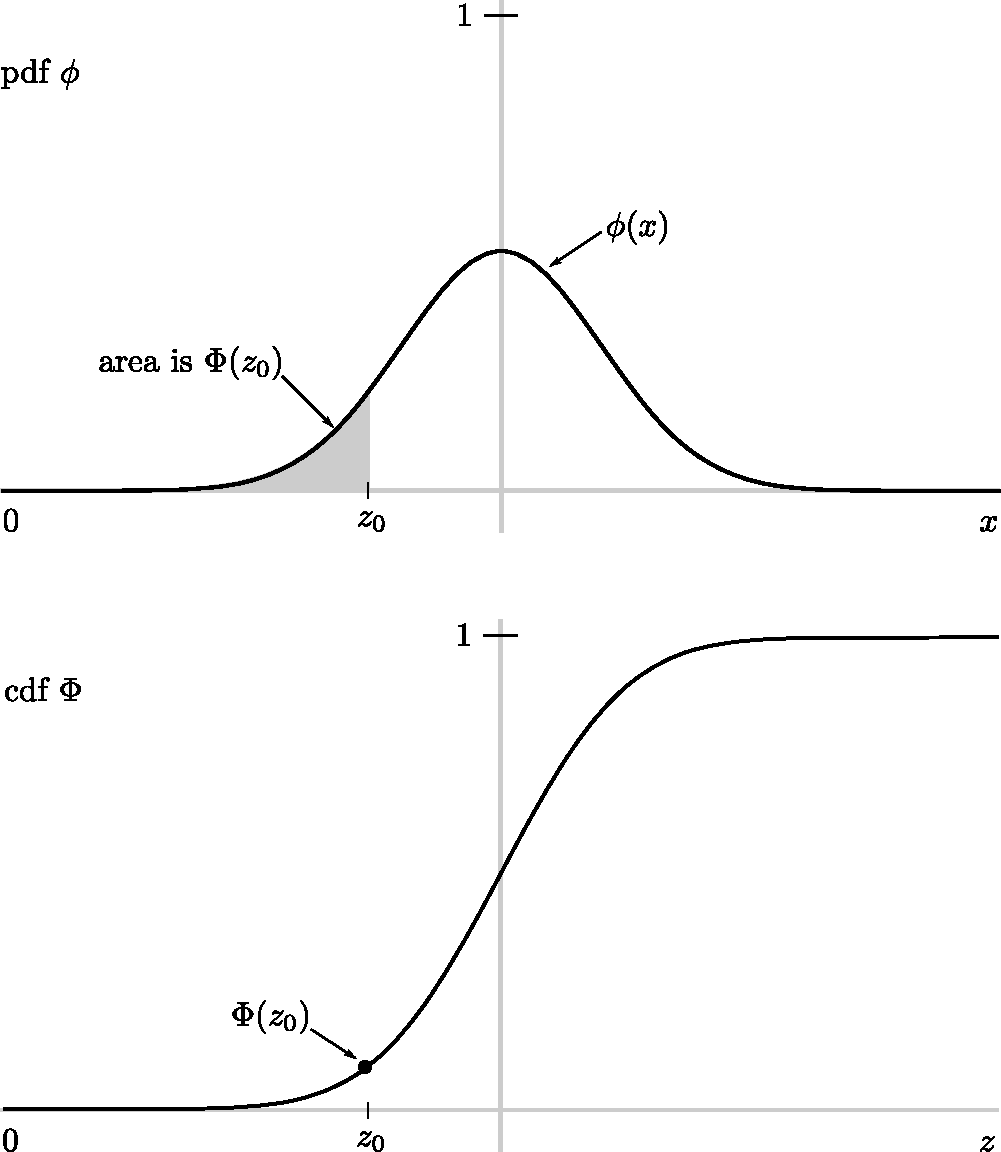
\includegraphics[scale=0.3]{figures/gaussian.pdf}}
\end{center}
\end{minipage}
\end{frame}

\begin{frame}[fragile]
\pause

\begin{framed}
\tiny gaussian.py: Accept floats $z$, $mu$, and $sigma$ as command-line arguments. Use them to test the \lstinline{phi()} and \lstinline{Phi()} functions. Write the results to standard output.
\end{framed}

\begin{lstlisting}[language=Python]
import math
import stdio
import sys

def pdf(x, mu = 0.0, sigma = 1.0):
    x = float(x - mu) / sigma
    return math.exp(- x * x / 2.0) / math.sqrt(2.0 * math.pi) / sigma

def cdf(z, mu = 0.0, sigma = 1.0):
    z = float(z - mu) / sigma
    if z < -8.0: return 0.0
    if z > +8.0: return 1.0
    total = 0.0
    term = z
    i = 3
    while total != total + term:
        total += term
        term *= z * z / i
        i += 2
    return 0.5 + total * pdf(z)
\end{lstlisting}
\end{frame}

\begin{frame}[fragile]
\pause

\begin{lstlisting}[language=Python]
def main():
    z = float(sys.argv[1])
    mu = float(sys.argv[2])
    sigma = float(sys.argv[3])
    stdio.writeln(cdf(z, mu, sigma))

if __name__ == '__main__':
    main()
\end{lstlisting}

\pause

\begin{lstlisting}[language={}]
$ python gaussian.py 820 1019 209
0.170509668691
$ python gaussian.py 1500 1019 209
0.989316483738
$ python gaussian.py 1500 1025 231
0.980122090737
\end{lstlisting}
\end{frame}

\section{Using Functions to Organize Code}

\begin{frame}[fragile]
\pause

\begin{framed}
\tiny coupon.py: Accept integer $n$ as a command-line argument. Write to standard output the number of coupons collected before obtaining one of each of $n$ types.
\end{framed}

\begin{lstlisting}[language=Python]
import random
import stdarray
import stdio
import sys

def getCoupon(n):
    return random.randrange(0, n)

def collect(n):
    found = stdarray.create1D(n, False)
    couponCount = 0
    distinctCouponCount = 0
    while distinctCouponCount < n:
        coupon = getCoupon(n)
        couponCount += 1
        if not found[coupon]:
            distinctCouponCount += 1
            found[coupon] = True
    return couponCount

def main():
    n = int(sys.argv[1])
    couponCount = collect(n)
    stdio.writeln(couponCount)

if __name__ == '__main__':
    main()
\end{lstlisting}
\end{frame}

\begin{frame}[fragile]
\pause

\begin{lstlisting}[language={}]
$ python coupon.py 1000
5193
$ python coupon.py 1000
6865
$ python coupon.py 1000000
15490879
\end{lstlisting}
\end{frame}

\section{Passing Arguments and Returning Values}
\begin{frame}[fragile]
\pause

We can use parameter variables anywhere in the body of the function in the same way as we use local variables

\pause
\bigskip

Python initializes the parameter variable with the corresponding argument provided by the calling code --- an approach known as call by object reference (aka call by value)

\pause
\bigskip

As a consequence, if a parameter variable refers to a mutable object and we change that object's value within a function, then this also changes the object's value in the calling code

\pause
\bigskip

For example, the following function exchanges the values in the list \lstinline{a} at indices \lstinline{i} and \lstinline{j}
\begin{lstlisting}[language=Python]
def exchange(a, i, j):
    temp = a[i]
    a[i] = a[j]
    a[j] = temp
\end{lstlisting}

\begin{lstlisting}[language=Python]
a = [1, 2, 3, 4, 5]
exchange(a, 1, 4) 
stdio.writeln(a)    # will output [1, 5, 3, 4, 2]
\end{lstlisting}
\end{frame}

\begin{frame}[fragile]
\pause

When a function takes a list as an argument, it typically implements a function that operates on an arbitrary number of objects

\pause
\bigskip

For example, the following function computes and returns the average value of the numbers in the list \lstinline{a}
\begin{lstlisting}[language=Python]
def mean(a):
    total = 0.0
    for v in a:
        total += v
    return total / len(a)
\end{lstlisting}

\pause
\bigskip

There are situations where it is useful for a function to return a list

\pause
\bigskip

For example, the following function returns a list containing \lstinline{n} random numbers, each between 0 and 1
\begin{lstlisting}[language=Python]
def randomarray(n):
    a = stdarray.create1D(n)
    for i in range(n):
        a[i] = random.random()
    return a
\end{lstlisting}
\end{frame}

\begin{frame}[fragile]
\pause

\begin{framed}
\tiny playthattunedeluxe.py: Read sound samples from standard input, add harmonics, and play the resulting sound to standard audio.
\end{framed}

\begin{lstlisting}[language=Python]
import math
import stdarray
import stdaudio
import stdio

def superpose(a, b, aWeight, bWeight):
    c = stdarray.create1D(len(a), 0.0)
    for i in range(len(a)):
        c[i] = a[i] * aWeight + b[i] * bWeight
    return c

def tone(hz, t):
    SPS = 44100
    n = int(SPS * t)
    a = stdarray.create1D(n + 1, 0.0)
    for i in range(n + 1):
        a[i] = math.sin(2.0 * math.pi * i * hz / SPS)
    return a

def note(pitch, t):
    CONCERT_A_HZ = 440.0
    NOTES_ON_SCALE = 12.0
    hz = CONCERT_A_HZ * (2.0 ** (pitch / NOTES_ON_SCALE))
    a = tone(hz, t)
    hi = tone(2 * hz, t)
    lo = tone(hz / 2, t)
    h = superpose(hi, lo, .5, .5)
    return superpose(a, h, .5, .5)
\end{lstlisting}
\end{frame}

\begin{frame}[fragile]
\pause

\begin{lstlisting}[language=Python]
def main():
    while not stdio.isEmpty():
        pitch = stdio.readInt()
        duration = stdio.readFloat()
        a = note(pitch, duration)
        stdaudio.playSamples(a)
    stdaudio.wait()

if __name__ == '__main__':
    main()
\end{lstlisting}

\pause

\begin{minipage}{170pt}
\begin{lstlisting}[language={}]
$ head -5 elise.txt
7 .125 
6 .125 
7 .125 
6 .125 
7 .125 
\end{lstlisting}

\pause

\begin{lstlisting}[language={}]
$ python playthattunedeluxe.py < elise.txt
\end{lstlisting}
\end{minipage}%
\begin{minipage}{130pt}
\hfill \visible<4->{\href{run:elisedeluxe.wav}{
\includegraphics[scale=0.2]{figures/speaker.png} \ExternalLink}}
\end{minipage}
\end{frame}

\section{Filter, Lambda, Map, and Reduce Functions}
\begin{frame}[fragile]
\pause

In Python, functions are first-class objects, meaning they are actually data just like numbers, lists, and strings

\pause
\bigskip

As a result, we can write functions that take other functions as arguments and return other functions as results

\pause
\bigskip

The built-in function \lstinline{filter(f, seq)} returns those items of the sequence \lstinline{seq} for which \lstinline{f(item)} is \lstinline{True}
\begin{lstlisting}[language={}]
>>> primes = filter(is_prime, range(11))
>>> primes
[2, 3, 5, 7]
\end{lstlisting}

\pause
\bigskip

A lambda function is a ``disposable'' function that we can define just when we need it and then immediately throw it away after we are done using it
\begin{lstlisting}[language={}]
>>> odds = filter(lambda x : x % 2 != 0, range(11))
>>> odds
[1, 3, 5, 7, 9]
\end{lstlisting}
\end{frame}

\begin{frame}[fragile]
\pause

The built-in function \lstinline{map(f, seq)} returns a list of the results of applying the function \lstinline{f} to the items of the sequence \lstinline{seq}
\begin{lstlisting}[language={}]
squares = map(lambda x : x ** 2, range(11))
>>> squares
[0, 1, 4, 9, 16, 25, 36, 49, 64, 81, 100]
\end{lstlisting}

\pause
\bigskip

The built-in function \lstinline{reduce(f, seq)} applies a function \lstinline{f} of two arguments cumulatively to the items of a sequence \lstinline{seq}, from left to right, so as to reduce the sequence to a single value
\begin{lstlisting}[language={}]
>>> total = reduce(lambda x, y: x + y, range(11))
>>> total
55
\end{lstlisting}
\end{frame}

\begin{frame}[fragile]
\pause

The RSA cryptosystem is the most widely-used public key cryptography algorithm in the world, which can be used to encrypt a message without the need to exchange a secret key separately

\pause
\bigskip

A message $x$ is encrypted using the function $f(x) = x^e \bmod n$, where $n=pq$ for two different large primes $p$ and $q$ chosen at random, and $e$ is a random prime number less than $m=(p-1)(q-1)$ such that $e$ does not divide $m$

\pause
\bigskip

The maximum number that can be encrypted is $n-1$

\pause
\bigskip

Together, the values $e$ and $n$ are called the public key

\pause
\bigskip

A message $y$ is decrypted using the function $g(y) = y^d \bmod n$, where $1 \leq d < m$ is the multiplicative inverse of $e \bmod m$, ie, $ed \bmod m = 1$

\pause
\bigskip

The value $d$ is called the private key
\end{frame}

\begin{frame}[fragile]
\pause

\begin{framed}
\tiny cryptography.py: A module that implements RSA cryptosystem.
\end{framed}

\begin{lstlisting}[language=Python]
import random
import stdio

def is_prime(N):
    if N < 2: 
        return False
    i = 2
    while i <= N / i:
        if N % i == 0:
            return False
        i += 1
    return True

def primes(N):
    return filter(is_prime, range(N))

def inverse(e, m):
    return filter(lambda d: e * d % m == 1, range(1, m))[0]

def make_encoder_decoder(N):
    p, q = random.sample(primes(N), 2)
    n = p * q
    m = (p - 1) * (q - 1)
    stdio.writef('Maximum number that can be encrypted is %d\n', n - 1)
    e = random.choice(primes(m))
    while m % e == 0:
        e = random.choice(primes(m))
    d = inverse(e, m)
    return [lambda x: (x ** e) % n, lambda y: (y ** d) % n]
\end{lstlisting}
\end{frame}

\begin{frame}[fragile]
\pause

\begin{lstlisting}[language={}]
>>> import cryptography
>>> encoder, decoder = cryptography.make_encoder_decoder(100)
Maximum number that can be encrypted is 2536
>>> encoder(42)
2235L
>>> decoder(2235)
42L
>>> decoder(encoder(1729))
1729L
\end{lstlisting}
\end{frame}
\end{document}
